 \section{Results}
For presenting some numerical result we wrote a program that simulates working cycle of the adaptive algorithm.
Our algorithm rotates homodyne angle for getting the best estimation by means of cancelling the back action. On Fig. \ref{alpha_10} (left) we can see, how homodyne angle depends on time.
\begin{figure}[t]
 \begin{minipage}{0.5\linewidth}
  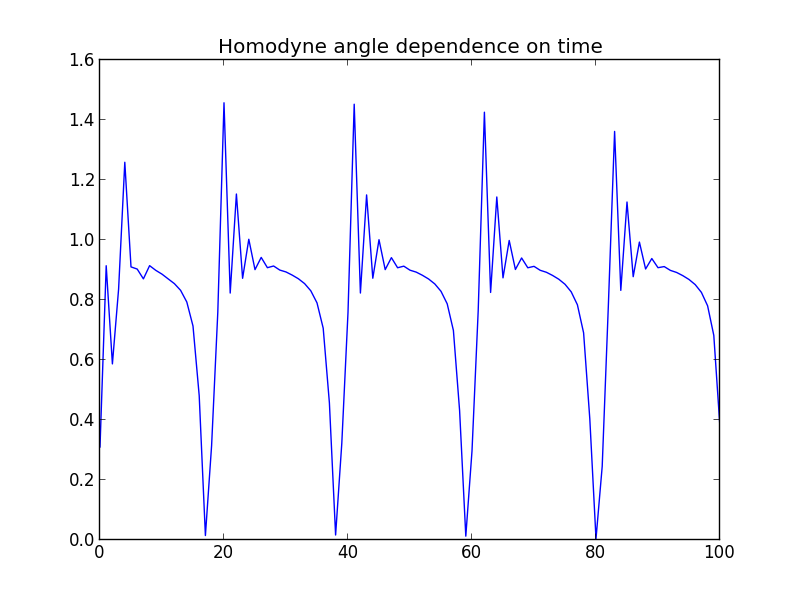
\includegraphics[width=1.\linewidth]{z_big_F}
 \end{minipage}
\hfill
 \begin{minipage}{0.5\linewidth}
  \center{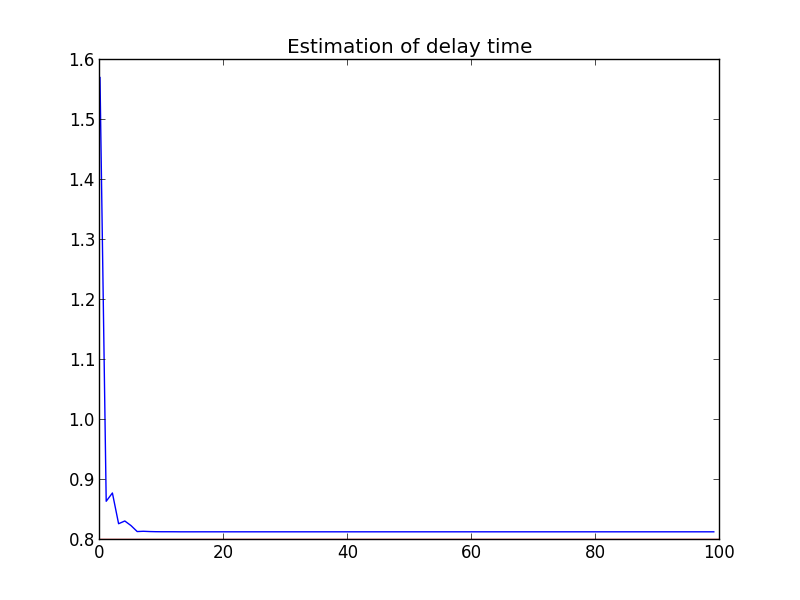
\includegraphics[width=1.\linewidth]{T_a10_big}}
 \end{minipage}
\caption{Homodyne angle $\zeta(t)$ dependence on time \textit{(left)} and estimation of delay time depending on time \textit{(right)}.}
\label{alpha_10}
 \end{figure}
Also we can see how our algorithm estimates the arrival time (See  Fig. \ref{alpha_10} (right)). Then for compartment we place how estimation algorithm works in adaptive measurements and in measurements with fixed homodyne angle (see Fig.\ref{FbAb}).
\begin{figure}[h]
 \begin{minipage}{0.5\textwidth}
  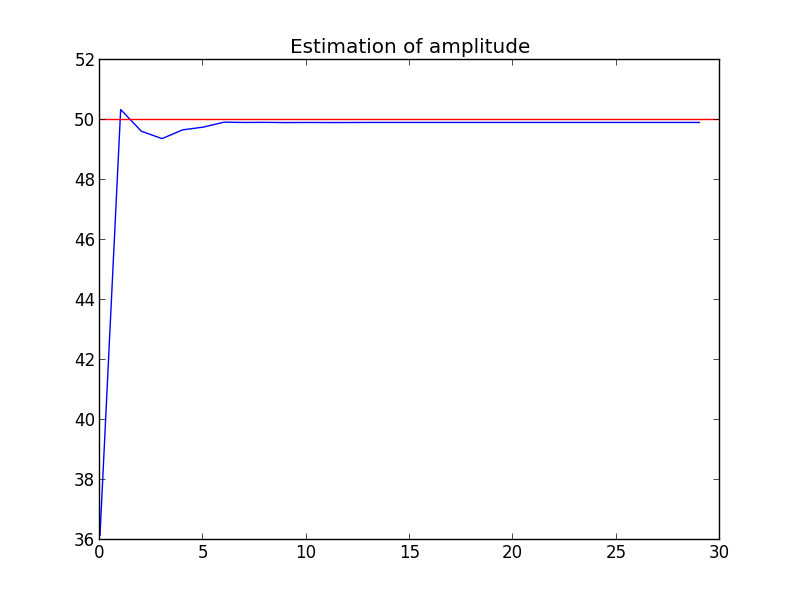
\includegraphics[width=1.\linewidth]{F_a10_big}
 \end{minipage}
\hfill
 \begin{minipage}{0.5\textwidth}
  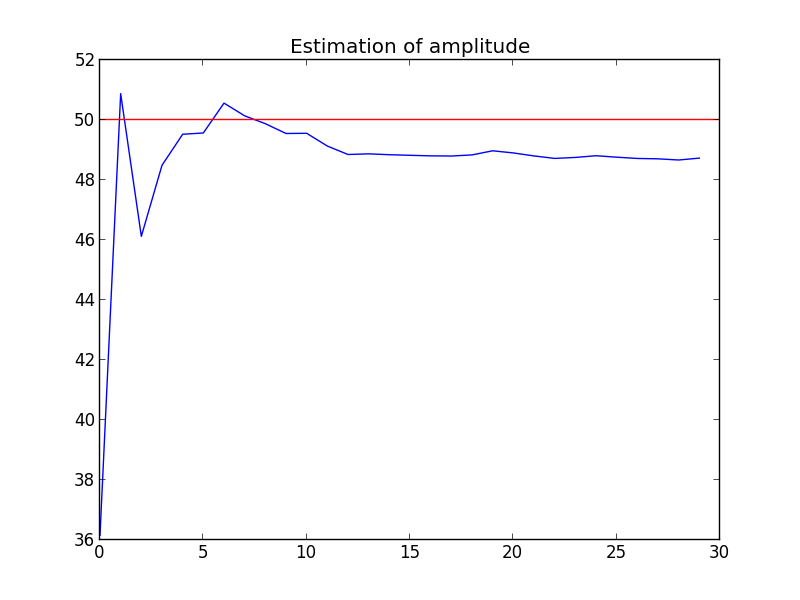
\includegraphics[width=1.\linewidth]{F_a10_big_ph}
 \end{minipage}
\caption{Compare the estimation of amplitude in adaptive measurements\textit(left) and measurements with fixed homodyne angle \textit{right}}
\label{FbAb}
\end{figure}
Finally we place here some numerical results (see Table \ref{set1}). All the results we discuss in the next section.
\begin{table}[h!]
 \center{\begin{tabular}{|c||c|c|c|c|}
  \hline
    & $\bar{F}_{est}$ & $\Delta F$ &  $\bar{\tau}_{est}$ & $\Delta \tau$\\
\hline
 Variational readout & -- & 0.0015 &  -- & -- \\
\hline
Adaptive measurement & 51.122 & 0.022 & 0.9 & 0.0004 \\
\hline
Fixed homodyne angle $\zeta = \pi/2$  & 51.035 & 0.064 & 0.9023 & 0.0023 \\
\hline
 \end{tabular}}
\caption{$\tau = 0.9, F = 51.1, N = 1000,T=6.6$}
\label{set1}
\end{table}